%\documentclass[UTF8]{ctexart} % use larger type; default would be 10pt
\documentclass[a4paper]{article}
\usepackage{xeCJK}
%\usepackage[utf8]{inputenc} % set input encoding (not needed with XeLaTeX)

%%% Examples of Article customizations
% These packages are optional, depending whether you want the features they provide.
% See the LaTeX Companion or other references for full information.

%%% PAGE DIMENSIONS
\usepackage{geometry} % to change the page dimensions
\geometry{a4paper} % or letterpaper (US) or a5paper or....
\geometry{margin=1in} % for example, change the margins to 2 inches all round
% \geometry{landscape} % set up the page for landscape
%   read geometry.pdf for detailed page layout information

\usepackage{graphicx} % support the \includegraphics command and options

% \usepackage[parfill]{parskip} % Activate to begin paragraphs with an empty line rather than an indent

%%% PACKAGES
\usepackage{booktabs} % for much better looking tables
\usepackage{array} % for better arrays (eg matrices) in maths
\usepackage{paralist} % very flexible & customisable lists (eg. enumerate/itemize, etc.)
\usepackage{verbatim} % adds environment for commenting out blocks of text & for better verbatim
\usepackage{subfig} % make it possible to include more than one captioned figure/table in a single float
% These packages are all incorporated in the memoir class to one degree or another...

%%% HEADERS & FOOTERS
\usepackage{fancyhdr} % This should be set AFTER setting up the page geometry
\pagestyle{fancy} % options: empty , plain , fancy
\renewcommand{\headrulewidth}{0pt} % customise the layout...
\lhead{}\chead{}\rhead{}
\lfoot{}\cfoot{\thepage}\rfoot{}

%%% SECTION TITLE APPEARANCE
\usepackage{sectsty}
\allsectionsfont{\sffamily\mdseries\upshape} % (See the fntguide.pdf for font help)
% (This matches ConTeXt defaults)

%%% ToC (table of contents) APPEARANCE
\usepackage[nottoc,notlof,notlot]{tocbibind} % Put the bibliography in the ToC
\usepackage[titles,subfigure]{tocloft} % Alter the style of the Table of Contents
\renewcommand{\cftsecfont}{\rmfamily\mdseries\upshape}
\renewcommand{\cftsecpagefont}{\rmfamily\mdseries\upshape} % No bold!

%%% END Article customizations

%%% The "real" document content comes below...

\setlength{\parindent}{0pt}
\usepackage{physics}
\usepackage{amsmath}
%\usepackage{symbols}
\usepackage{AMSFonts}
\usepackage{bm}
%\usepackage{eucal}
\usepackage{mathrsfs}
\usepackage{amssymb}
\usepackage{float}
\usepackage{multicol}
\usepackage{abstract}
\usepackage{empheq}
\usepackage{extarrows}
\usepackage{textcomp}
\usepackage{fontspec}
\usepackage{braket}
\usepackage{siunitx}
\sisetup{
	separate-uncertainty = true,
	inter-unit-product = \ensuremath{{}\cdot{}}
}
\usepackage{mhchem}
\usepackage{hyperref}
\hypersetup{
	colorlinks=true,
	linkcolor=black,
	filecolor=magenta,      
	urlcolor=cyan,
}

\DeclareMathOperator{\p}{\prime}
\DeclareMathOperator{\ti}{\times}
\DeclareMathOperator{\intinf}{\int_0^\infty}
\DeclareMathOperator{\intdinf}{\int_{-\infty}^\infty}
\DeclareMathOperator{\intzpi}{\int_0^\pi}
\DeclareMathOperator{\intztpi}{\int_0^{2\pi}}
\DeclareMathOperator{\sumninf}{\sum_{n=1}^{\infty}}
\DeclareMathOperator{\sumninfz}{\sum_{n=0}^\infty}
\DeclareMathOperator{\sumiinf}{\sum_{i=1}^{\infty}}
\DeclareMathOperator{\sumiinfz}{\sum_{i=0}^\infty}
\DeclareMathOperator{\sumkinf}{\sum_{k=1}^{\infty}}
\DeclareMathOperator{\sumkinfz}{\sum_{k=0}^\infty}
\DeclareMathOperator{\e}{\mathrm{e}}
\DeclareMathOperator{\I}{\mathrm{i}}
\DeclareMathOperator{\Arg}{\mathrm{Arg}}
\newcommand{\NA}{N_\mathrm{A}}
\newcommand{\kB}{k_\mathrm{B}}

\DeclareMathOperator{\ra}{\rightarrow}
\DeclareMathOperator{\llra}{\longleftrightarrow}
\DeclareMathOperator{\lra}{\longrightarrow}
\DeclareMathOperator{\dlra}{\Leftrightarrow}
\DeclareMathOperator{\dra}{\Rightarrow}
\newcommand{\bkk}[1]{\Braket{#1|#1}}
\newcommand{\bk}[2]{\Braket{#1|#2}}
\newcommand{\bkev}[2]{\Braket{#2|#1|#2}}



\DeclareMathOperator{\hV}{\hat{\vb{V}}}

\DeclareMathOperator{\hx}{\hat{\vb{x}}}
\DeclareMathOperator{\hy}{\hat{\vb{y}}}
\DeclareMathOperator{\hz}{\hat{\vb{z}}}

\DeclareMathOperator{\hA}{\hat{\vb{A}}}

\DeclareMathOperator{\hQ}{\hat{\vb{Q}}}
\DeclareMathOperator{\hI}{\hat{\vb{I}}}
\DeclareMathOperator{\psis}{\psi^\ast}
\DeclareMathOperator{\Psis}{\Psi^\ast}
\DeclareMathOperator{\hi}{\hat{\vb{i}}}
\DeclareMathOperator{\hj}{\hat{\vb{j}}}
\DeclareMathOperator{\hk}{\hat{\vb{k}}}
\DeclareMathOperator{\hr}{\hat{\vb{r}}}
\DeclareMathOperator{\hT}{\hat{\vb{T}}}
\DeclareMathOperator{\hH}{\hat{H}}
\DeclareMathOperator{\hh}{\hat{h}}               % helicity
\DeclareMathOperator{\hL}{\hat{\vb{L}}}
\DeclareMathOperator{\hp}{\hat{\vb{p}}}

\DeclareMathOperator{\ha}{\hat{\vb{a}}}
\DeclareMathOperator{\hS}{\hat{\vb{S}}}
\DeclareMathOperator{\hSigma}{\hat{\bm\Sigma}}
\DeclareMathOperator{\hJ}{\hat{\vb{J}}}
\DeclareMathOperator{\hP}{\hat{\vb{P}}}          % Parity
\DeclareMathOperator{\hC}{\hat{\vb{C}}} 
\DeclareMathOperator{\Tdv}{-\dfrac{\hbar^2}{2m}\dv[2]{x}}
\DeclareMathOperator{\Tna}{-\dfrac{\hbar^2}{2m}\nabla^2}
\DeclareMathOperator{\vna}{\vnabla}
\DeclareMathOperator{\nna}{\nabla^2}
\newcommand{\naCarExpd}[1]{\pdv[2]{#1}{x} + \pdv[2]{#1}{y} + \pdv[2]{#1}{z}}
\newcommand{\naCyl}{\qty[\dfrac{1}{\rho}\pdv{\rho}\qty(\rho\pdv{\rho}) + \dfrac{1}{\rho^2}\pdv[2]{\phi} + \pdv[2]{z}]}

%\DeclareMathOperator{\g#0}{\gamma^0}
%\DeclareMathOperator{\g1}{\gamma^1}
%\DeclareMathOperator{\g2}{\gamma^2}
%\DeclareMathOperator{\g3}{\gamma^3}
%\DeclareMathOperator{\g5}{\gamma^5}
\newcommand{\g}[1]{\gamma^{#1}}
\DeclareMathOperator{\gmuu}{\gamma^\mu}
\DeclareMathOperator{\gmud}{\gamma_\mu}
%\newcommand{\G}[2]{g^{#1#2}}

\newcommand{\subsbul}{\subsection*{$ \bullet $}}
\newcommand{\ex}[1]{\paragraph{18-#1}}
\newcommand{\subex}[1]{\subparagraph{#1}}
\newcommand{\dis}{\displaystyle}
\newcommand{\iden}{{\large \bm{1}}}
\newcommand{\qed}{$ \Square $}
\newcommand{\tPhi}{\tilde{\Phi} }
\DeclareMathOperator{\au}{\mathrm{a.u.}}
\newcommand{\ntg}{\notag\\}

\numberwithin{equation}{section}
%\setcounter{secnumdepth}{4}
\setcounter{tocdepth}{4}
%\allowdisplaybreaks[4]

\usepackage{xcolor}
\definecolor{codegray}{gray}{0.9}
\newfontfamily\Consolas{Consolas}
\newcommand{\code}[1]{\colorbox{codegray}{{\Consolas#1}}}

\title{\textbf{Advanced Physical Chemistry II}\\HW}
\author{王石嵘
\vspace{5pt}\\
161240065\\
%Email: shirong\_wang@berkeley.edu
}
\date{\today} % Activate to display a given date or no date (if empty),
         % otherwise the current date is printed 

\begin{document}
% \boldmath

\maketitle

%\tableofcontents

%\newpage

\setcounter{section}{17}
\section{Partition Functions and Ideal Gases}
5,8,13,16,20,24,29,32,38\\
\ex{5}
\begin{equation}\label{key}
f_2 = \dfrac{2\e^{-\beta E_2}}{2 + 2\e^{-\beta E_2} + 4\e^{-\beta E_3} + 2\e^{-\beta E_4}}
\end{equation}
where
\begin{align}
E_2 &= \SI{14903.66}{cm^{-1}}\\
E_3 &= \SI{14904.00}{cm^{-1}}\\
E_4 &= \SI{27206.12}{cm^{-1}}\\
\beta & = \dfrac{1}{\SI{0.6950}{cm^{-1}.K^{-1}}\times T}
\end{align}
thus
\begin{align}
f_2(300K) & = \num{9.05e-32}\\
f_2(1000K) &= \num{4.86e-10}\\
f_2(2000K) &= \num{2.20e-5}
\end{align}

\ex{8}
\begin{align}
\Theta_{vib}(\ce{H_2}) &= \dfrac{hc\tilde{\nu}_{\ce{H_2}}}{\kB} = \dfrac{\SI{6.626e-34}{J.s}\cdot \SI{2.998e10}{cm.s^{-1}}\cdot \SI{4401}{cm^{-1}}}{\SI{1.381e-23}{J.K^{-1}}} = \SI{6330}{K}\\
\Theta_{vib}(\ce{D_2}) &= \dfrac{hc\tilde{\nu}_{\ce{D_2}}}{\kB} = \dfrac{\SI{6.626e-34}{J.s}\cdot \SI{2.998e10}{cm.s^{-1}}\cdot \SI{3112}{cm^{-1}}}{\SI{1.381e-23}{J.K^{-1}}} = \SI{4476}{K}
\end{align}

\ex{13}
Since
\begin{equation}\label{key}
\varepsilon_J = \dfrac{\hbar^2 J(J+1)}{2I} = \kB T
\end{equation}
thus
\begin{equation}\label{key}
J(J+1) = \dfrac{2I \kB T}{\hbar^2} = \dfrac{T}{\Theta_{rot}} 
\end{equation}
For $ \ce{N_2} $(g) at $ \SI{300}{K} $,
\begin{equation}\label{key}
J(J+1) = \dfrac{300}{2.88} = 104.167
\end{equation}
thus
\begin{equation}\label{key}
J = 9.72\approx 10
\end{equation}

\ex{16}
\begin{align}
\sum_{v=0}^\infty \e^{-\beta(v+1/2)h\nu} &= \e^{-\Theta_{vib}(v+1/2)/T} = \e^{-\Theta_{vib}/2T} \sum_{v=0}^\infty \e^{-\Theta_{vib} v/T} 
\end{align}
Let
\begin{equation}\label{key}
f(v) = \e^{-\Theta_{vib} v/T} 
\end{equation}
we have
\begin{align}
f'(v) &= -\dfrac{\Theta_{vib}}{T}\e^{-\Theta_{vib} v/T} \notag\\
f'''(v) &= -\qty(\dfrac{\Theta_{vib}}{T})^3 \e^{-\Theta_{vib} v/T} 
\end{align}
thus
\begin{align}
\sum_{v=0}^\infty \e^{-\beta(v+1/2)h\nu} &= \e^{-\Theta_{vib}/2T} \qty[\intinf \e^{-\Theta_{vib} v/T} \dd v + \dfrac{1}{2}(1-0) - \dfrac{1}{12}\qty(-\dfrac{\Theta_{vib}}{T} - 0) + \dfrac{1}{720}\qty(\qty(-\dfrac{\Theta_{vib}}{T})^3 - 0) + \mathcal{O}(T^{-3})] \notag\\
&= \e^{-\Theta_{vib}/2T} \qty[\dfrac{T}{\Theta_{vib}} + \dfrac{1}{2} + \dfrac{1}{12}\dfrac{\Theta_{vib}}{T} +  \mathcal{O}(T^{-3})] 
\end{align}
For $ O_2 $, $ \Theta_{vib} = \SI{2256}{K} $, thus
\begin{equation}\label{key}
q_{vib} = \e^{-2256/600}\qty(\dfrac{300}{2256} + \dfrac{1}{2} + \dfrac{1}{12}\dfrac{2256}{300}) = 0.0293
\end{equation}
while
\begin{equation}\label{key}
q_{vib}(\text{exact}) = \dfrac{\e^{-2256/600}}{1 - \e^{-2256/300}} = 0.0233
\end{equation}
thus the error is about $ 26\% $.

\ex{20}
Eq. 18.41 gives
\begin{equation}\label{key}
\dfrac{\bar{C}_V}{R} = \dfrac{5}{2} + \dfrac{\Theta_{vib}^2}{T^2}\dfrac{\e^{-\Theta_{vib} /T}}{(1 - \e^{-\Theta_{vib} /T})^2}
\end{equation}
where $ \Theta_{vib} = \SI{3103}{K} $ for $ \ce{CO} $(g).\\
thus the theoretical and experimental curve are as follows
\begin{figure}[H]
	\centering
	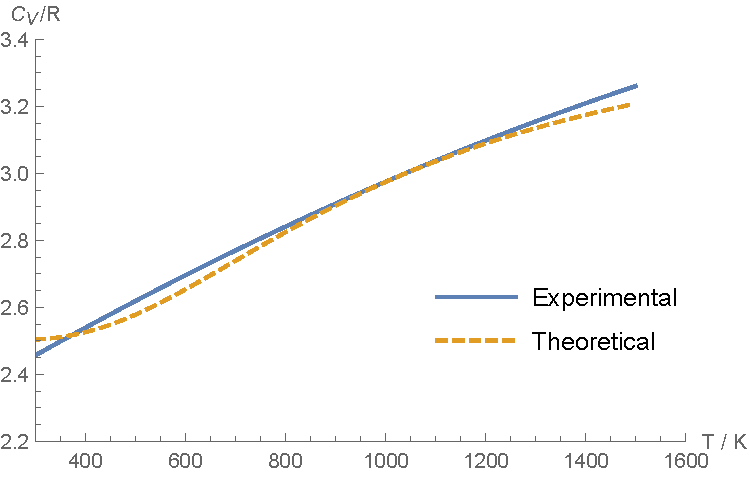
\includegraphics[width=0.65\linewidth]{18-20.pdf}
\end{figure}

\ex{24}
\begin{equation}\label{key}
\Theta_{rot} = \dfrac{\hbar^2}{2I \kB} = \dfrac{(\SI{1.045e-34}{J.s})^2}{2\times \SI{18.816e-47}{kg.m^2}\times\SI{1.381e-23}{J.K^{-1}}} = \SI{2.10}{K}
\end{equation}
\begin{align}
\Theta_{vib,1} &= \dfrac{hc\tilde{\nu}_1}{\kB} = \dfrac{\SI{6.626e-34}{J.s}\times\SI{2.998e10}{cm.s^{-1}} \times\SI{2096.7}{cm^{-1}}}{\SI{1.381e-23}{J.K^{-1}}} = \SI{3016}{K} \\
\Theta_{vib,2} &= \dfrac{hc\tilde{\nu}_1}{\kB} = \dfrac{\SI{6.626e-34}{J.s}\times\SI{2.998e10}{cm.s^{-1}} \times\SI{713.46}{cm^{-1}}}{\SI{1.381e-23}{J.K^{-1}}} = \SI{1026}{K} \\
\Theta_{vib,3} &= \dfrac{hc\tilde{\nu}_1}{\kB} = \dfrac{\SI{6.626e-34}{J.s}\times\SI{2.998e10}{cm.s^{-1}} \times\SI{3311.47}{cm^{-1}}}{\SI{1.381e-23}{J.K^{-1}}} = \SI{4763}{K} 
\end{align}
Since $ \ce{HCN} $ is linear
\begin{align}
\dfrac{\bar{C}_V(\SI{3000}{K})}{R} &= \dfrac{5}{2} + \sum_j g_j\dfrac{\Theta_{vib}^2}{T^2}\dfrac{\e^{-\Theta_{vib} /T}}{(1 - \e^{-\Theta_{vib} /T})^2} \notag\\
&= \dfrac{5}{2} + \qty(\dfrac{3016}{3000})^2\dfrac{\e^{-3016/3000}}{(1-\e^{-3016/3000})^2} + 2\qty(\dfrac{1026}{3000})^2\dfrac{\e^{-1026/3000}}{(1-\e^{-1026/3000})^2} + \qty(\dfrac{4763}{3000})^2\dfrac{\e^{-4763/3000}}{(1-\e^{-4763/3000})^2} \notag\\
&= 6.214
\end{align}
thus
\begin{equation}\label{key}
\bar{C}_V(\SI{3000}{K}) = 6.214R
\end{equation}

\ex{29}
\begin{align}
\Theta_{vib,1} &= \dfrac{hc\tilde{\nu}_1}{\kB} = \dfrac{\SI{6.626e-34}{J.s}\times\SI{2.998e10}{cm.s^{-1}} \times\SI{1319.7}{cm^{-1}}}{\SI{1.381e-23}{J.K^{-1}}} = \SI{1898}{K} \\
\Theta_{vib,2} &= \dfrac{hc\tilde{\nu}_1}{\kB} = \dfrac{\SI{6.626e-34}{J.s}\times\SI{2.998e10}{cm.s^{-1}} \times\SI{749.8}{cm^{-1}}}{\SI{1.381e-23}{J.K^{-1}}} = \SI{1078}{K} \\
\Theta_{vib,3} &= \dfrac{hc\tilde{\nu}_1}{\kB} = \dfrac{\SI{6.626e-34}{J.s}\times\SI{2.998e10}{cm.s^{-1}} \times\SI{1617.75}{cm^{-1}}}{\SI{1.381e-23}{J.K^{-1}}} = \SI{2327}{K} 
\end{align}
\begin{align}
\Theta_{rot,A} &= \dfrac{hc\tilde{\nu}_1}{\kB} = \dfrac{\SI{6.626e-34}{J.s}\times\SI{2.998e10}{cm.s^{-1}} \times\SI{8.0012}{cm^{-1}}}{\SI{1.381e-23}{J.K^{-1}}} = \SI{11.51}{K} \\
\Theta_{rot,B} &= \dfrac{hc\tilde{\nu}_1}{\kB} = \dfrac{\SI{6.626e-34}{J.s}\times\SI{2.998e10}{cm.s^{-1}} \times\SI{0.43304}{cm^{-1}}}{\SI{1.381e-23}{J.K^{-1}}} = \SI{0.623}{K} \\
\Theta_{rot,C} &= \dfrac{hc\tilde{\nu}_1}{\kB} = \dfrac{\SI{6.626e-34}{J.s}\times\SI{2.998e10}{cm.s^{-1}} \times\SI{0.41040}{cm^{-1}}}{\SI{1.381e-23}{J.K^{-1}}} = \SI{0.590}{K} 
\end{align}

\begin{align}
\dfrac{\bar{C}_V(\SI{1000}{K})}{R} &= 3 + \sum_j g_j\dfrac{\Theta_{vib}^2}{T^2}\dfrac{\e^{-\Theta_{vib} /T}}{(1 - \e^{-\Theta_{vib} /T})^2} \notag\\
&= 3 + \qty(\dfrac{1898}{1000})^2\dfrac{\e^{-1898/1000}}{(1-\e^{-1898/1000})^2} + \qty(\dfrac{1078}{1000})^2\dfrac{\e^{-1078/1000}}{(1-\e^{-1078/1000})^2} + \qty(\dfrac{2327}{1000})^2\dfrac{\e^{-2327/1000}}{(1-\e^{-2327/1000})^2} \notag\\
&= 3 + 0.747 + 0.908 + 0.649 \notag\\
&= 5.30
\end{align}
thus
\begin{equation}\label{key}
\bar{C}_V(\SI{1000}{K}) = 5.30R
\end{equation}

\newpage
\ex{32}
The theoretical heat capacity is
\begin{equation}\label{key}
\dfrac{\bar{C}_V}{R} = 3 + \sum_j^9 \dfrac{\Theta_{vib,j}^2}{T^2}\dfrac{\e^{-\Theta_{vib,j}/T}}{(1 - \e^{-\Theta_{vib,j} /T})^2}
\end{equation}
where
\begin{align}
\Theta_{vib,1} &= \SI{4170}{K} \notag\\
\Theta_{vib,2} &= \Theta_{vib,3} = \SI{2180}{K} \notag\\
\Theta_{vib,4} &= \Theta_{vib,5} = \Theta_{vib,6} = \SI{4320}{K} \notag\\
\Theta_{vib,7} &= \Theta_{vib,8} = \Theta_{vib,9} = \SI{1870}{K} 
\end{align}
thus the theoretical and experimental curve are as follows
\begin{figure}[H]
	\centering
	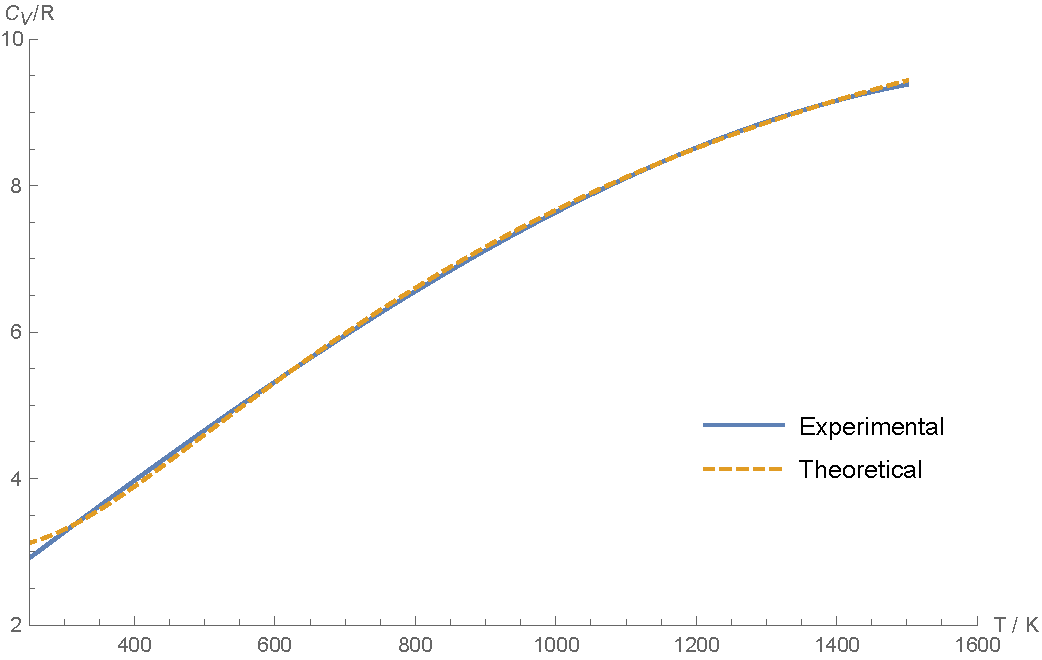
\includegraphics[width=0.7\linewidth]{18-32.pdf}
\end{figure}


\ex{38}
A 2-dimensional diatomic molecule has 2 translational degrees of freedom, 1 vibrational degrees of freedom, 1 rotational degrees of freedom. Thus, in total, 4 degrees of freedom.\\
The rotational partition function is
\begin{align}
q_{rot} &= \dfrac{1}{\sigma}\intinf g_J \e^{-\epsilon_J/\kB T}\dd J \notag\\
&=  \dfrac{1}{\sigma}\intinf g_J \e^{-\Theta_{rot} J^2/T}\dd J \notag\\
&= \sqrt{\dfrac{\pi T}{\Theta_{rot}}}
\end{align}
while
\begin{align}
q_{trans} &= \dfrac{2a^2\pi m \kB T}{h^2} \\
q_{vib} &= \dfrac{\e^{-\Theta_{vib}/2T}}{1 - \e^{-\Theta_{vib} /T}}
\end{align}
thus
\begin{equation}\label{key}
q(T) = \dfrac{2a^2\pi m \kB T}{h^2} \sqrt{\dfrac{\pi T}{\Theta_{rot}}} \dfrac{\e^{-\Theta_{vib}/2T}}{1 - \e^{-\Theta_{vib} /T}}
\end{equation}
thus
\begin{align}
\ev{E} &= N\kB T^2 \qty(\pdv{\ln q}{T})_V \notag\\
&= N\kB T^2 \pdv{\qty[\ln T + \dfrac{1}{2}\ln T - \dfrac{\Theta_{vib}}{2T} - \ln(1-\e^{-\Theta_{vib} /T})]}{T} \notag\\
&= N\kB T^2 \qty[\dfrac{3}{2}\dfrac{1}{T} + \dfrac{\Theta_{vib}}{2T^2} + \dfrac{\e^{-\Theta_{vib} /T}}{1-\e^{-\Theta_{vib} /T}}\dfrac{\Theta_{vib}}{T^2}] \notag\\
&= N\kB \qty[\dfrac{3}{2}T + \dfrac{\Theta_{vib}}{2} + \Theta_{vib}\dfrac{\e^{-\Theta_{vib} /T}}{1-\e^{-\Theta_{vib} /T}}] 
\end{align}




\end{document}